\section{Ch. 3 (AO)}
\subsection{Problem 3.3.1}

Suppose that the internal force $F_\text{int}$ due to molecular collisions has no systematic part $F_\text{sys}$ (i.e., there is no damping term $\propto v(t)$). Then $F_\text{int}=\eta(t)$. \textbf{Goal:} Work through the steps of this chapter once again in this case, to show we then get
\begin{equation}
\overline{v(t)} = v_0,~\overline{v^2(t)} = v_0^2 + \frac{\Gamma t}{m^2}.
\end{equation}

Consider the differential equation
\begin{equation}
m \dot{v}(t) = \underbrace{-m \gamma v(t) + \eta(t)}_{=F_\text{int}} + F_\text{ext}(t)
\end{equation}
when $\gamma=0$, $F_\text{ext}(t)=0$. The formal solution to this differential equation is
\begin{equation}
v(t) = v_0 + \frac{1}{m} \int_{0}^{t} \eta(t') dt'
\end{equation}
Performing a conditional average over different realizations of the noise (assuming the tagged particles initial velocity is $v_0$) yields
\begin{eqnarray}
\overline{v(t)}&=& \underbrace{\overline{v_0}}_{=v_0} + \frac{1}{m} \int_{0}^{t} \underbrace{\overline{\eta(t')}}_{=0} dt' \\
&=& v_0.
\end{eqnarray}
Performing the same average over $v^2(t)$ gives
\begin{eqnarray}
\overline{v^2(t)}&=& \overline{v_0^2} + \frac{2 v_0 }{m} \int_{0}^{t} \overline{\eta(t')} dt' + \frac{1}{m^2} \int_{0}^{t} dt_1 \int_{0}^{t} dt_2 \overline{\eta(t_1) \eta(t_2)}  \\
&=& v_0^2 + \frac{\Gamma}{m^2} \int_{0}^{t} dt_1 \int_{0}^{t} dt_2 \delta(t_1-t_2) \\
&=& \boxed{v_0^2 + \frac{\Gamma}{m^2} \int_{0}^{t} dt_1 = v_0^2 + \frac{\Gamma t}{m^2}},
\end{eqnarray}
where the last line follows from the assumption that $\overline{\eta(t_1) \eta(t_2)}=\Gamma \delta(t_1-t_2)$ (the noise has a correlation time of zero).

\subsection{Problem 3.3.2}

Again assume there is no internal damping but that
\begin{equation}
\overline{\eta(t_1) \eta(t_2)} = K \exp(-|t_1-t_2|/\tau).
\end{equation}
\textbf{Goal:} Determine the long-time behavior of $\overline{v^2(t)}$.

Assuming $\overline{\eta(t)}=0$, it is immediately clear that $\overline{v(t)}=v_0$ which is clearly incorrect. For pedagogical purposes we will compute $\overline{v^2(t)}$ and analyze the expression in some relevant limiting cases.

Let us begin by breaking the rectangular integration area into two regions: (i) $t_1>t_2$ and (ii) $t_1 < t_2$. Notice that in region (i) our correlation function is given by 
\begin{equation}
\overline{\eta(t_1) \eta(t_2)}_{(i)} = K \exp(-(t_1-t_2)/\tau)
\end{equation}
and in region (ii) it is given by 
\begin{equation}
\overline{\eta(t_1) \eta(t_2)}_{(ii)} = K \exp(-(t_2-t_1)/\tau).
\end{equation}
From here it follows that
\begin{eqnarray}
\overline{v^2(t)}&=& \overline{v_0^2} + \frac{2 v_0 }{m} \int_{0}^{t} \overline{\eta(t')} dt' + \frac{1}{m^2} \int_{0}^{t} dt_1 \int_{0}^{t} dt_2 \overline{\eta(t_1) \eta(t_2)} \nonumber \\
&=& v_0^2 + \frac{K}{m^2} \int_{0}^{t} dt_1 \int_{0}^{t} dt_2 \exp(-|t_1-t_2|/\tau) \nonumber \\
&=& v_0^2 + \frac{K}{m^2} \int_{0}^{t} dt_1 \times \bigg\{ \int_{0}^{t_1} dt_2 \exp(-(t_1-t_2)/\tau) \nonumber \\ &+& \int_{t_1}^{t} dt_2 \exp(-(t_2-t_1)/\tau)\bigg\} \nonumber \\
&=& v_0^2 + \frac{K}{m^2} \bigg\{ \tau \bigg(t + \tau \exp(-t_1/\tau)\bigg) \bigg|_{0}^{t} - \tau \bigg(\tau \exp((t_1-t)/\tau)-t\bigg) \bigg|_{0}^{t} \bigg\} \nonumber \\
&=& \boxed{v_0^2 + \frac{K}{m^2} \bigg\{ 2 \tau t  + 2 \tau^2 \exp(-t/\tau) -2 \tau^2 \bigg\}}~.
\end{eqnarray}
For $t\ll\tau$, this reduces to $v_0^2+K t^2 / m^2$ which grows quadratically with $t$ -- this is the `balistic' regime. For $t\gg \tau$, this reduces to $v_0^2+2K \tau t / m^2$ which grows linearly in $t$ -- this is the `diffusive' regime.


\subsection{Problem 3.3.3}

Instead of the very specific decaying exponential form in problem 3.2, suppose you are given only that
\begin{itemize}
\item[(i)] $\overline{\eta(t_1) \eta(t_2)}$ is a function of $|t_1-t_2|$, the magnitude of the 
time difference between the two time arguments
\item[(ii)] $\overline{\eta(t_1) \eta(t_2)}$ tends to zero as $|t_1-t_2|\rightarrow\infty$.
\end{itemize}
\textbf{Goal:} Show that the inescapable conclusion based on properties (i) and (ii) is that $\overline{v^2(t)}$ increases linearly with $t$ at long times, in the absence of a damping term $\gamma$.

In what follows, we will denote the $\overline{\eta(t_1) \eta(t_2)}$ by $f(|t_1-t_2|)$. Notice that the argument of $f$ is identically zero $\forall~t_1=t_2$. Let us use this fact to break the integral below into two equal parts:
\begin{eqnarray}
(\overline{v^2(t)}-v_0^2) \times m^2 &=& \int_{0}^{t} dt_1 \int_{0}^{t} dt_2 ~ f(|t_1-t_2|) \nonumber \\
&=& \bigg\{\underbrace{\int_{0}^{t} dt_1 \int_{0}^{t_1} dt_2}_{=T_1} + \underbrace{\int_{0}^{t} dt_1 \int_{t_1}^{t} dt_2}_{=T_2} \bigg\} f(|t_1-t_2|)\label{eq:eq3p3},
\end{eqnarray}
where $T_1$ and $T_2$ correspond to the triangular-shaped integration domains shown in Fig. \ref{fig:3p3}. To show that these two integrals are equal, consider a displacement from the line $t_2=t_1$, given by $(t_1-\Delta t, t_1+\Delta t)$. Evaluating $f$ at this point yields $f(|-\Delta t-\Delta t|)=f(|2\Delta t|)$. Similarly, we can evaluate $f$ at the point $(t_1+\Delta t, t_1-\Delta t)$, which also yields $f(|+\Delta t+\Delta t|)=f(|2\Delta t|)$. Clearly then, the integrals over each of these domains are equal. To show this using calculus, let us reverse the order of integration in the second term in Eq. (\ref{eq:eq3p3}), which yields
\begin{eqnarray}
(\overline{v^2(t)}-v_0^2) \times m^2
&=& \bigg\{\underbrace{\int_{0}^{t} dt_1 \int_{0}^{t_1} dt_2}_{=T_1} + \underbrace{\int_{0}^{t} dt_2 \int_{0}^{t_2} dt_1}_{=T_2} \bigg\} f(|t_1-t_2|)  \nonumber \\
&=& 2 \int_{0}^{t} dt_1 \int_{0}^{t_1} dt_2 ~f(|t_1-t_2|).  \nonumber \\
\end{eqnarray}
The second line follows from the fact that we can interchange labels for $t_1$ and $t_2$ in the second integral, as these are just dummy variables. Now one has that
\begin{eqnarray}
(\overline{v^2(t)}-v_0^2) \times m^2 &=& 2 \int_{0}^{t} dt_1 \int_{t_1}^{0} -dt' ~f(|t'|)  \nonumber \\ 
&=& 2 \int_{0}^{t} dt_1 \int_{0}^{t_1} dt' ~f(|t'|)  \nonumber \\ 
&=& 2 \int_{0}^{t} dt'~f(|t'|) \int_{t'}^{t_1} dt_1  \nonumber \\ 
&=& 2 \int_{0}^{t} dt'~ (t-t')f(|t'|).
\end{eqnarray}
This result was obtained by substituting $t'=t_1-t_2$ and then reversing the order of integration for integrals over $dt_1$ and $dt'$. Assuming $f(|t'|)$ decays over some characteristic timescale $\tau$, for $t\gg \tau$ , we have that 
\begin{eqnarray}
(\overline{v^2(t)}-v_0^2) \times m^2 &=& 2 \int_{0}^{t} dt'~ (t-t')f(|t'|) \\
&=& 2 t \bigg( \int_{0}^{t} dt'~ f(|t'|) - \int_{0}^{t} dt'~ \frac{t'}{t} f(|t'|)\bigg)\\
& \simeq & 2t \int_{0}^{t} dt'~ f(|t'|),
\end{eqnarray}
as the second term is subdominate until $t'\sim t$, but then $f(|t'|) \rightarrow 0$ since $t'\sim t>>\tau$. As an example, consider $f(|t'|)=C \exp(t'/\tau)$. The integral above equates to $2C(t \tau - \tau^2)$.
\begin{figure}[h]
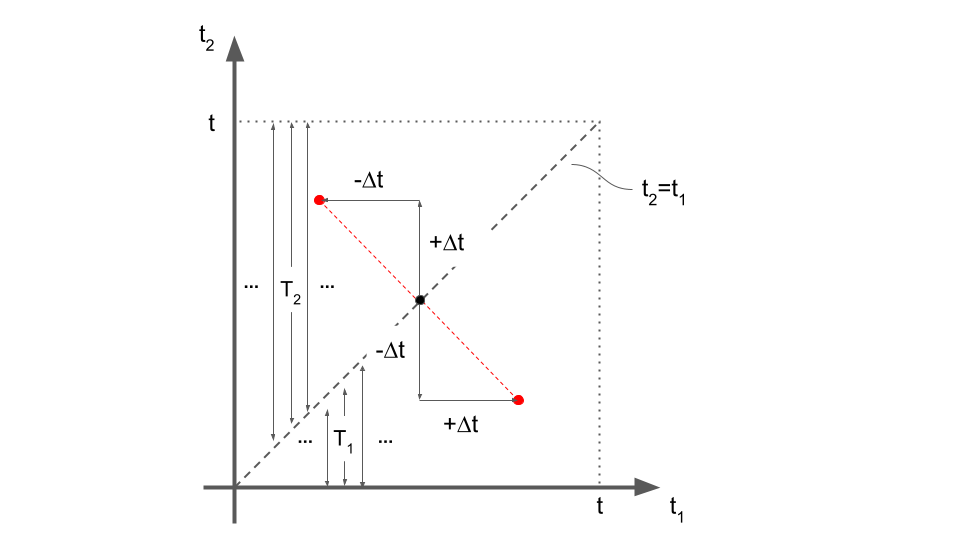
\includegraphics[width=16cm]{fig_problem_3p3.png}
    \caption{Symmetry of the integration domain for the integral $ \int_{0}^{t} dt_1 \int_{0}^{t} dt_2 ~ f(|t_1-t_2|)$.}
    \label{fig:3p3}
\end{figure}